\documentclass[10pt,a4paper]{article}

%------- packges ---------_%
% author's contact footnote
\usepackage{authblk}
% math tools
\usepackage{amsmath}
%\numberwithin{equation}{section} %enable this to include section in equation
\usepackage{amsfonts}
\usepackage{amssymb}
\usepackage{amsthm}
\usepackage{mathtools}
\usepackage{mathrsfs}
% making hyperlinks blue
\usepackage[hidelinks]{hyperref}
\hypersetup{bookmarksopen=true}
\usepackage{xcolor}
\hypersetup{
	colorlinks,
	linkcolor={red!50!black},
	citecolor={blue!50!black},
	urlcolor={blue!80!black}
}
%bib also backref and blue
\usepackage{enotez}
\setenotez{backref}
\usepackage{listings}
\usepackage{xcolor}

%code syntax hightlight
\definecolor{codegreen}{rgb}{0,0.6,0}
\definecolor{codegray}{rgb}{0.5,0.5,0.5}
\definecolor{codepurple}{rgb}{0.58,0,0.82}
\definecolor{backcolour}{rgb}{0.95,0.95,0.92}

\lstdefinestyle{mystyle}{
    backgroundcolor=\color{backcolour},   
    commentstyle=\color{codegreen},
    keywordstyle=\color{magenta},
    numberstyle=\tiny\color{codegray},
    stringstyle=\color{codepurple},
    basicstyle=\ttfamily\footnotesize,
    breakatwhitespace=false,         
    breaklines=true,                 
    captionpos=b,                    
    keepspaces=true,                 
    numbers=left,                    
    numbersep=5pt,                  
    showspaces=false,                
    showstringspaces=false,
    showtabs=false,                  
    tabsize=2
}

\lstset{style=mystyle}


%convenience
%mathbb
\def\R{\mathbb R}
\def\N{\mathbb N}
\def\E{\mathbb E}
\def\P{\mathbb P}

%mathcal
\def\cP{\mathcal P}
\def\cS{\mathcal S}
\def\cX{\mathcal X}
\def\cY{\mathcal Y}
\def\cA{\mathcal A}
\def\cB{\mathcal B}
\def\cW{\mathcal W}

%mathbf
\def\1{\mathbf 1}
\def\0{\mathbf 0}
\def\A{\mathbf A}
\def\B{\mathbf B}
\def\C{\mathbf C}
\def\D{\mathbf D}
\def\E{\mathbf E}
\def\M{\mathbf M}
\def\N{\mathbb N}
\def\O{\mathbf O}
\def\P{\mathbf P}
\def\Q{\mathbf Q}
\def\R{\mathbb R}
\def\S{\mathbf S}
\def\T{\mathbf T}
\def\a{\mathbf a}
\def\b{\mathbf b}
\def\c{\mathbf c}
\def\e{\mathbf e}
\def\F{\mathbf F}
\def\G{\mathbf G}
\def\H{\mathbf H}
\def\h{\mathbf h}
\def\g{\mathbf g}
\def\m{\mathbf m}
\def\p{\mathbf p}
\def\q{\mathbf q}
\def\r{\mathbf r}
\def\s{\mathbf s}
\def\t{\mathbf t}
\def\u{\mathbf u}
\def\v{\mathbf v}
\def\U{\mathbf U}
\def\w{\mathbf w}
\def\x{\mathbf x}
\def\y{\mathbf y}
\def\Y{\mathbf Y}
\def\z{\mathbf z}
\def\Z{\mathbb Z}

%figure setting
\usepackage{graphicx}
\usepackage{subcaption}
\usepackage{bookmark}

% TITLE
\author{Quang-Thanh Tran}
\title{Advanced Macroeconomics: HW1}

%================== MAIN ====================%
\begin{document}
\maketitle
\section{Deriving the Steady State}
	The Social Planner problem is
	\begin{align}
		\max_{c_t, k_{t+1}} &\sum^{\infty}_{t=0} \beta^t \ln(c_t) \\
		\text{s.t. } \  \label{eq:cons_c} c_t + k_{t+1} &= k_t^\alpha + (1-\delta)k_t, \\
		c_t &\geq 0, \nonumber \\
		k_{t+1} &\geq 0, \nonumber \\
		k_0 &\geq 0 \nonumber \text{given}.
	\end{align}
From \eqref{eq:cons_c}, $c_t$ can be expressed as
\begin{equation}
	\label{eq:c} c_t = k_t^\alpha - k_{t+1} + (1-\delta)k_t.
\end{equation}
The Bellman equation is
\begin{align}
	\label{eq:bellman} V(k_t) = \max_{c_t, k_{t+1}} \left[ \ln(c_t) + \beta V(k_{t+1}) \right].
\end{align}
Plugging \eqref{eq:c} into \eqref{eq:bellman}, the problem becomes
\begin{align}
	\label{eq:bellman2} V(k_t) = \max_{k_{t+1}} \ln(k_t^\alpha - k_{t+1} + (1-\delta)k_t) + \beta V(k_{t+1}).
\end{align}
The optimal solution must be true for any $t$. To find the optimal $k_{t+1}$, taking the FOC with respect to $k_{t+1}$ yields
\begin{align}
	\frac{\partial V(k_t)}{\partial k_{t+1}} = \frac{-1}{k_t^\alpha - k_{t+1} + (1-\delta)k_t} + \beta \frac{\partial V(k_{t+1})}{\partial k_{t+1}} = 0. \nonumber
\end{align}
so that
\begin{equation}
	\label{eq:preeuler} \beta \frac{\partial V(k_{t+1})}{\partial k_{t+1})} = \frac{1}{k_t^\alpha - k_{t+1} + (1-\delta)k_t} \left(\equiv \frac{1}{c_t} \right).
\end{equation}
To find $\partial V(k_{t+1})/ k_{t+1}$, first, differentiate \eqref{eq:bellman2} wrt $k_t$ 
\begin{align}
	\frac{\partial V(k_t)}{\partial k_t} = \frac{\alpha k_t^{\alpha-1} + (1-\delta)}{k_t^\alpha - k_{t+1} + (1-\delta)k_t},
\end{align}
implying that
\begin{equation}
	 \frac{V(k_{t+1})}{k_{t+1}} = \frac{\alpha k_{t+1}^{\alpha-1} + (1-\delta)}{k_{t+1}^\alpha - k_{t+2} + (1-\delta)k_{t+1}} \left(\equiv \frac{\alpha k_{t+1}^{\alpha-1} + (1-\delta)}{c_{t+1}} \right).
\end{equation}
Plugging this equation back to \eqref{eq:preeuler} yields the Euler equation
\begin{equation}
	\label{eq:euler} \frac{c_{t+1}}{c_t} = \beta [\alpha k_{t+1}^{\alpha-1} + (1-\delta)].
\end{equation}
The equilibrium is reached when $c_t = c_{t+1} = c^{ss}$, where we set \eqref{eq:euler} equal 1. Thus, the steady-state capital stock $k^{ss}$ must satisfy
\begin{equation*}
	\beta [\alpha (k^{ss})^{\alpha-1} + (1-\delta)] = 1.
\end{equation*} 
Solving for $k^{ss}$
\begin{equation}
	\label{eq:kss} k^{ss} = \left(\frac{\alpha\beta}{1-\beta + \delta \beta }\right)^{1/(1-\alpha)}.
\end{equation}
If $\delta=1$, then we have
\begin{equation}
	k^{ss} = (\alpha\beta)^{1/(1-\alpha)}.
\end{equation}

\section{Solving Analytically: Guess and Verify}
\subsection{Policy Function}
A reasonable guess is that the Social Planner consumes a constant fraction of output each period. Suppose that the policy function has the following form
\begin{equation}
	\label{eq:policy_c} c_t = \sigma k_t^\alpha.
\end{equation}
We want to find an analytical expression for $\sigma$. Let $\delta=1$, plugging \eqref{eq:policy_c} into \eqref{eq:euler}, we have
\begin{equation}
	\frac{k^\alpha_{t+1}}{k^\alpha_t} = \alpha \beta k_{t+1}^{\alpha-1}.
\end{equation}
Rearranging and we obtain
\begin{equation}
	\label{eq:valf_k1} k_{t+1} = \alpha\beta k_t^\alpha.
\end{equation}
Putting this equation to the budget constraint \eqref{eq:cons_c} to obtain
\begin{equation}
	\label{eq:valf_c1} c_t = (1-\alpha\beta)k_t^\alpha,
\end{equation}
which implies that $\sigma = 1-\alpha\beta$.

\subsection{Value Function}
Since the utility function is a natural $\log$ form, we make a guess that the Value function takes the following form
\begin{equation}
	\label{eq:guess} V(k_t) = A + B \ln(k_t).
\end{equation}
Plugging into the Bellman equation \eqref{eq:bellman2}, we can rewrite the problem as
\begin{equation}
	\label{eq:bellman3} V(k_t) = \max_{c_t, k_{t+1}} \ln(c_t) + \beta [A + B\ln(k_{t+1})].
\end{equation}
We need to find the optimal values for \eqref{eq:bellman3} subject to the constraint \eqref{eq:cons_c}. With $\delta=1$, the Lagrangian is
\begin{equation}
	\mathcal{L} = \ln(c_t) + \beta [A + B\ln(k_{t+1})] + \lambda_t (k_t^\alpha - k_{t+1} - c_t).
\end{equation}
The first-order conditions are
\begin{align}
	& \label{eq:val_c} (c_t): \frac{1}{c_t} = \lambda_t, \\
	& \label{eq:val_k} (k_{t+1}): \frac{\beta B}{k_{t+1}} = \lambda_t.
\end{align}
From \eqref{eq:val_c} and \eqref{eq:val_k}, we then derive the Euler equation
\begin{equation}
	k_{t+1} = \beta B c_t.
\end{equation} 
Replacing $c_t$ from \eqref{eq:cons_c}, we obtain
\begin{equation}
	k_{t+1} = \beta B (k_t^\alpha - k_{t+1}).
\end{equation}
This implies
\begin{align}
	&\label{eq:sol_kt+1} k_{t+1} = \frac{\beta B}{1+\beta B} k_t^\alpha, \\
	&\label{eq:solc} c_t = \frac{1}{1+\beta B} k_t^\alpha \ \ \text{(from \eqref{eq:val_c})}.
\end{align}
By plugging these 2 expressions into the Value function at \eqref{eq:bellman3}, we have
\begin{equation*}
	V(k_t) = \ln \left( \frac{1}{1+\beta B} k_t^\alpha \right) + \beta \left[ A + B\ln\left(\frac{\beta B}{1+\beta B} k_t^\alpha \right) \right].
\end{equation*}
We can rearrange it to match our guess at \eqref{eq:guess}
\begin{equation}
	\label{eq:correct_value} V(k_t) = \underbrace{\left[ \beta(A + B\ln(\beta B)) - (1+\beta B)\ln(1+\beta B) \right]}_{A} + \underbrace{\alpha (1+\beta B)}_{B}\ln(k_t).
\end{equation}
With some algebra, we can solve for $A$ and $B$ as
\begin{align}
& \label{eq:sol_A} A = \frac{\alpha\beta}{(1-\alpha\beta)(1-\beta)}\ln(\alpha\beta) + \frac{1}{1-\beta}\ln(1-\alpha\beta), \\
& \label{eq:sol_B} B = \frac{\alpha}{1-\alpha\beta}.
\end{align}
Plugging \eqref{eq:sol_A}, \eqref{eq:sol_B} to equations \eqref{eq:sol_kt+1} and \eqref{eq:solc}, we have
\begin{align}
& \label{eq:valf_c2} c_t = (1-\alpha\beta)k_t^\alpha, \\
& \label{eq:valf_k2} k_{t+1} = \alpha \beta k_t^\alpha.
\end{align}
Note that \eqref{eq:valf_c2} is the same with \eqref{eq:valf_c1}, and \eqref{eq:valf_k2} is the same with \eqref{eq:valf_k1} so the two methods are consistent.

\section{Numerical Methods}

\subsection{Value Function Iteration}
Let us see how the algorithm works by reviewing the Bellman equation at \eqref{eq:bellman2}
\begin{equation*}
	V(k_t) = \max_{k_{t+1}} \ln(k_t^\alpha - k_{t+1} + (1-\delta)k_t) + \beta V(k_{t+1}). \tag{5}
\end{equation*}

\verb|Loop 1:| We first make an initial guess of $V^{(0)}(k_{t+1}) = 0$. Plugging back to \eqref{eq:bellman2} yields
\begin{equation*}
	V^{(1)}(k_t) = \max_{k^{(0)}_{t+1}} \ln(k_t^\alpha + (1-\delta) k_t) + 0.
\end{equation*}
Using this initial guess, $k^{(0)}_{t+1}$ is obviously 0 and we then find the value of $k_t$ that satisfies
\begin{equation*}
	V^{(1)}(k_t) = \ln(k_t^\alpha),
\end{equation*}
which implies that
\begin{equation*}
	V^{(1)} (k_t) = \alpha \ln(k_t).
\end{equation*}
Compared to \eqref{eq:correct_value}, this is far from the true value, but more accurate than the initial guess. We will use this updated value function, plug back again to \eqref{eq:bellman2} and do it again. 

\verb|Loop 2:| The next iteration yields
\begin{equation*}
	V^{(2)} (k_t) = \max_{k^{(1)}_{t+1}} \ln (k_t^\alpha - k_{t+1} + (1-\delta)k_t) + \beta \alpha \ln(k_{t+1}).
\end{equation*}
The FOC is:
\begin{equation*}
	-\frac{1}{k_t^\alpha - k_{t+1} + (1-\delta)k_t} + \alpha \beta \frac{1}{k_{t+1}} = 0.
\end{equation*}
Solving for $k_{t+1}$ yields (in MATLAB, we use \verb|fmindbnd| to find the maximizer).
\begin{equation*}
	k_{t+1} = \frac{\alpha\beta}{1+\alpha\beta} \left( k_t^\alpha + (1-\delta)k_t\right)
\end{equation*}
\textbf{From now on, let us assume that $\delta=1$}. We use this value and plug back to \eqref{eq:bellman2}
\begin{align*}
	V^{(2)} (k_t) &= \ln \left(k_t^\alpha - \frac{\alpha\beta}{1+\alpha\beta}k_t^\alpha \right) + \beta\alpha \ln\left( \frac{\alpha\beta}{1+\alpha\beta} k_t^\alpha \right) \\
	&= \underbrace{\ln\left(1-\frac{\alpha\beta}{1+\alpha\beta}\right) + \alpha\beta\ln\left(\frac{1}{1+\alpha\beta}\right)}_{\text{a constant}} + \alpha (1+\alpha\beta)\ln(k_t).
\end{align*}

\verb|Loop n:| If we repeat this process long enough, we will reach 
\begin{equation*}
	V^{(n)}(k_{t}) = \text{ some constant } + \underbrace{\alpha (1+\alpha\beta + (\alpha\beta)^2 + \dots )}_{\to \frac{\alpha}{1-\alpha\beta} \text{ as } n \to \infty} \ln(k_t).
\end{equation*}
which share a similar form to the true value function at \eqref{eq:correct_value}. Assuming that this is true, we can work out the policy function by inserting the true estimated value function to \eqref{eq:bellman2} and solve for $k_{t+1}$ to derive the policy function
\begin{equation*}
	k_{t+1} = \frac{\alpha\beta + (\alpha\beta)^2 + \dots}{1 + \alpha\beta + (\alpha\beta)^2 + \dots} k^\alpha_t \to \alpha\beta k_t^\alpha.
\end{equation*}


\subsection{The Code}
A popular numerical method is iterating the value function. First, since we already know the steady state of $k$ from \eqref{eq:kss}, we can construct a grid of possible values of $k$. In this case, the number of grid points is 100, and the $k$ candidates range from $0.5 k^{ss}$ to $2 k^{ss}$.

\begin{lstlisting}[language=Octave]
% initiate grid 
kmin = 0.5*kss;
kmax = 2*kss;
kgrid = 100; %no of grid points
kmat = linspace(kmin, kmax, kgrid); %make an array
kmat = kmat'; %convert to column vector
[N,n] = size(kmat);
\end{lstlisting}


At some iteration $n$, we have some estimate of the value function $V^{(n)}$. We then use the Bellman equation to compute the updated estimate of the value function $V^{(n+1)}$. Such iteration rule is expressed as follows
\begin{equation}
	V^{(n+1)}(k_t) = \max_{k_{t+1}} \left[ u(k_t^\alpha - k_{t+1} + (1-\delta)k_t) + \beta V^{(n)}(k_{t+1})  \right].
\end{equation}
The algorithm should eventually converge as demonstrated in the previous section.
For simplicity, let us set the initial value for $V^{(0)} = 0$.

\begin{lstlisting}[language=Octave]
tol = 0.0001;
maxiter = 300;
dif = tol+1000;
iter = 0;
% guess
v0 = zeros(N,1);
\end{lstlisting}

If we calculate the difference (or the distance in the vector space) between $V^{(1)}$ and $V^{(0)}$, then it would be
\begin{equation}
	d = \| V^{(1)}_i - V^{(0)}_i \|.
\end{equation}
Convergence means that $d \to 0 \approx \text{tol}$. This is when we stop the loop. 

The algorithm follows the iteration explained in the previous section. For each value of $k$, we find the $k_{t+1}$ that maximizes the Bellman equation given the initial guess of the value function. 
\begin{lstlisting}[language=Octave]
while dif > tol & iter < maxiter
	for i = 1:N
		k0 = kmat(i,1);
		k1 = fminbnd(@valfun, kmin, kmax);
		v1(i,1) = -valfun(k1); %because k1 is returned as negative
		kt(i,1) = k1;
	end
dif = norm(v1-v0);
v0 = v1;
iter = iter + 1;
end
\end{lstlisting}

For each spot $i$ in the state space, we get a \verb|k0| from the grid. Then line 4 searches and returns the \verb|k1| that maximizes the Bellman equation, which is stored in the file \verb|valfun.m|. Line 5 then collects the optimized value and calculates the new value function \verb|v1| while line 6 stores this \verb|k1| as the policy function. After the code loops over the possible values of the state, we calculate the difference and update the value function for the next loop.


If we use the function \verb|fminbnd|, it will search over all values of $k_1$ between \verb|kmin| and \verb|kmax|, including the points not in the original capital grid. Although doing so will help us find the true value function more accurately, the computation will take forever to complete. An alternative approach is a linear interpolation. We approximate the initial guess of the value function for points off the capital grid by producing a straight line.  
\begin{equation}
	V(k) \approx V(k(i)) + \frac{V(k(i+1)) - V(k(i))}{k(i+1) - k(i)} (k - k(i))
\end{equation}
By feeding the newly founded maximizer \verb|k1| into the linear interpolation of the value function, we can approximate the value function. Since the value function is an increasing function of $k$, we can narrow down the search after each loop.

\begin{lstlisting}[language=Octave]
function val=valfun(k)
    global v0 beta delta alpha kmat k0 kgrid
    ki0 = max(sum(k>kmat), 1); %identify the grid that falls just below the choice for k
    ki1 = ki0 + 1;
    %interpolation algorithm
    g = v0(ki0) + (k-kmat(ki0))*(v0(ki1)-v0(ki0))/(kmat(ki1)-kmat(ki0));
    % another interpolation algorithm
    %g = interp1(kmat, v0, k, 'linear');
    c = k0^alpha - k + (1-delta)*k0; %consumption
    if c <= 0
        val = -888-800*abs(c);
    else
        val = log(c) + beta*g;
    end
    %change value to negative since "fminbnd" finds minimum 
val = -val;
\end{lstlisting}

There are 2 ways to perform the interpolation. The first is optimizing the selection of the next $k$ candidate given our own algorithm. The second is to perform interpolation on the whole grid by using MATLAB \verb|interp1| function. The time to run the first is 4.336054 seconds, while the latter is 5.954239 seconds. Thus, we conclude that optimizing grid selection can improve efficiency.

\subsection{Read more}
\begin{itemize}
	\item The code: \url{https://github.com/thanhqtran/advanced_macroeconomics}
	\item Eric Sims' Note: \url{https://www3.nd.edu/~esims1/val_fun_iter.pdf}
	\item Ramsey model: Solving with value function iteration \url{https://www.youtube.com/watch?v=oYVfEXAbWEU}
	\item McCandless, G. (2008). The ABCs of RBCs: An introduction to dynamic macroeconomic models. Harvard University Press.
\end{itemize}


\newpage
\subsection{Figures}
With $\delta=1$:

\begin{figure}[ht]
\centering
\begin{subfigure}[b]{0.49\linewidth}
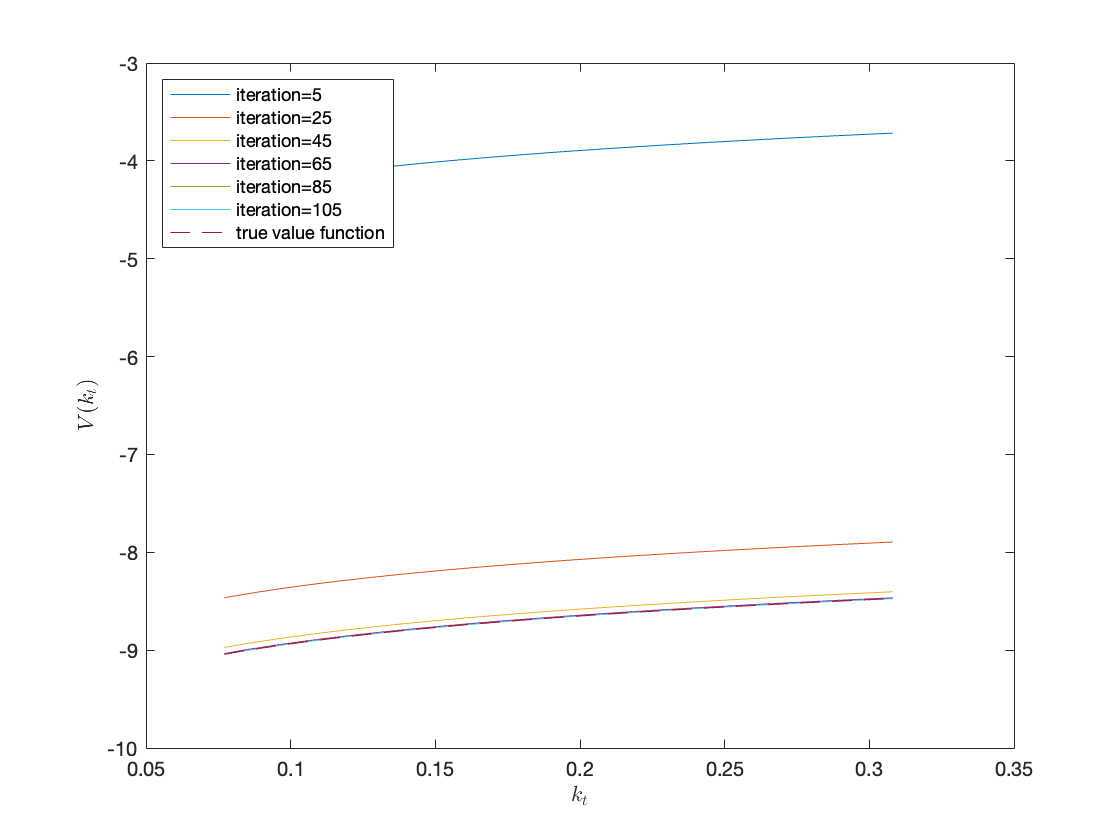
\includegraphics[width=\linewidth]{figs/delta1valfun.png}
\caption{Value function}
\end{subfigure}
\begin{subfigure}[b]{0.49\linewidth}
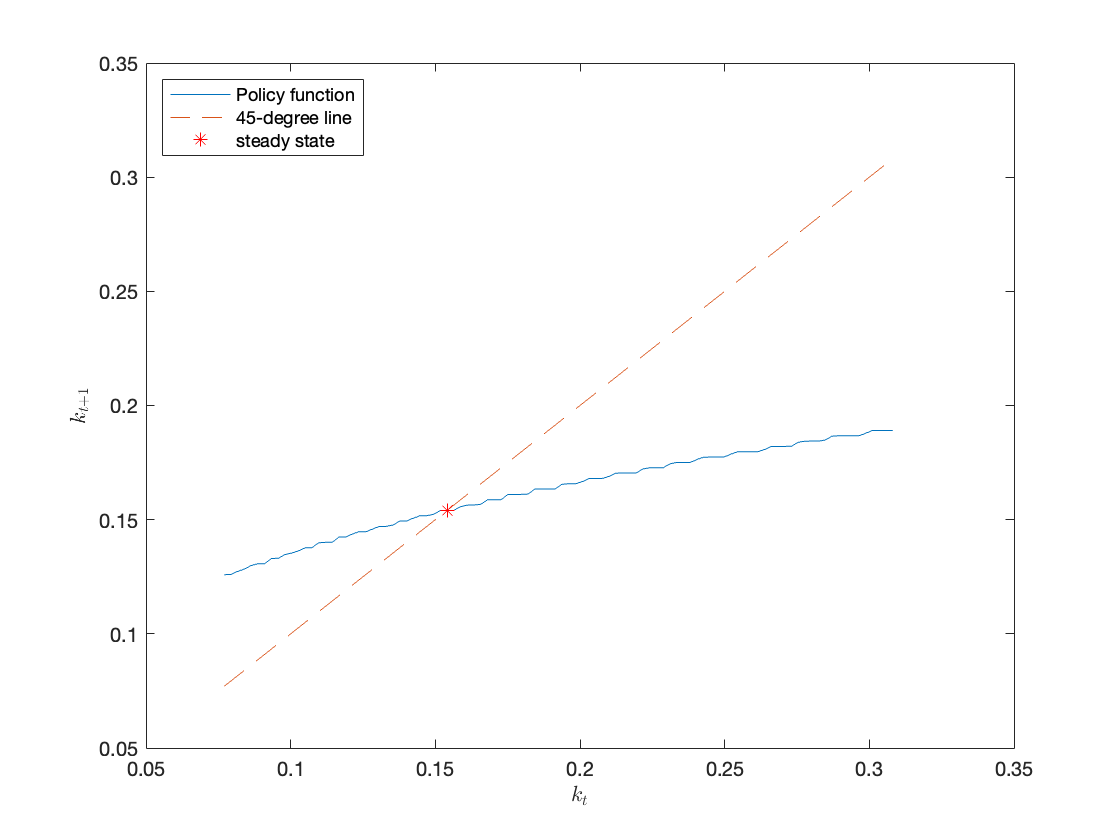
\includegraphics[width=\linewidth]{figs/delta1policyfun.png}
\caption{Policy function}
\end{subfigure}
\caption{The algorithms when $\delta=1$.}
\label{fig:delta1}
\end{figure}

With $\delta=0.1$:
\begin{figure}[ht]
\centering
\begin{subfigure}[b]{0.49\linewidth}
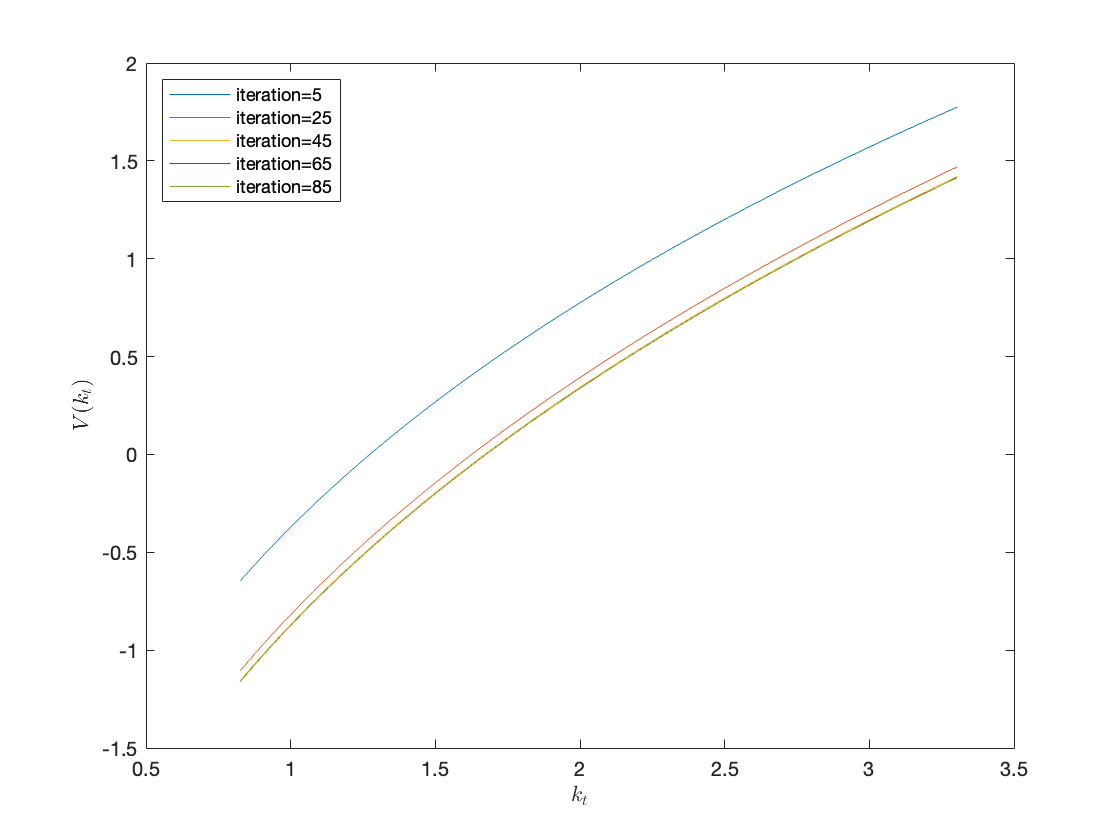
\includegraphics[width=\linewidth]{figs/delta01valfun.png}
\caption{Value function}
\end{subfigure}
\begin{subfigure}[b]{0.49\linewidth}
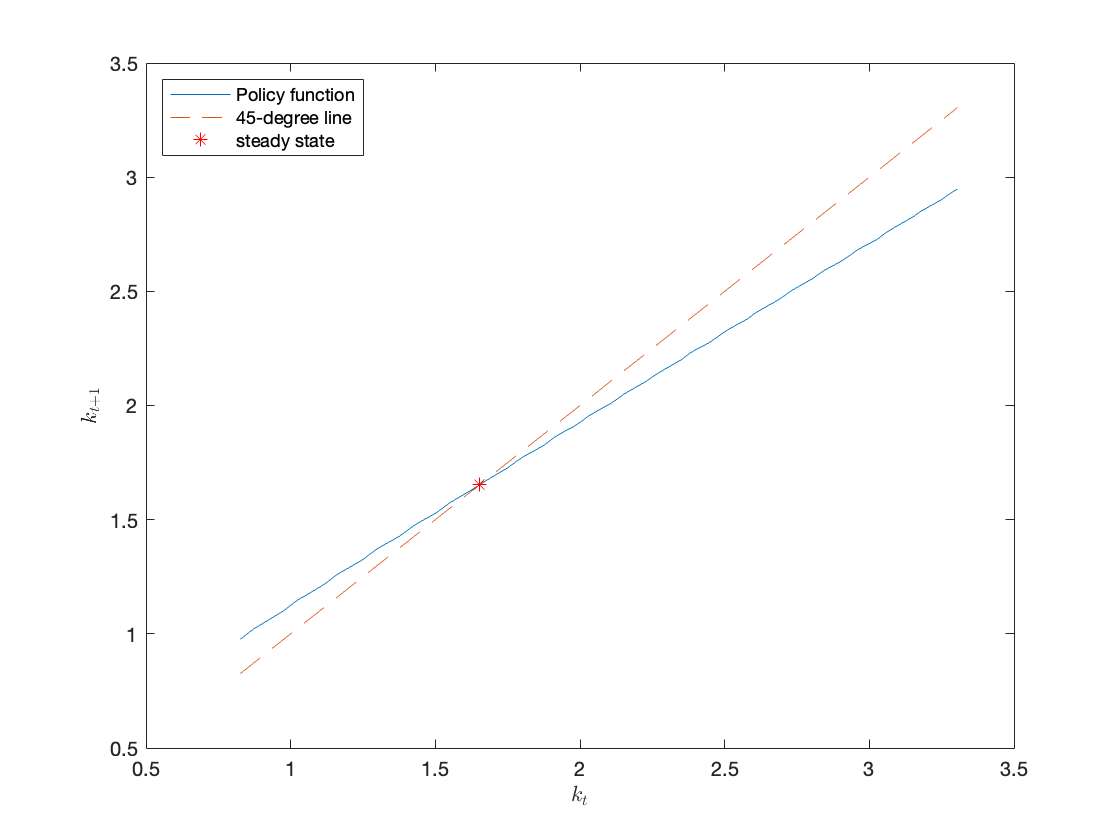
\includegraphics[width=\linewidth]{figs/delta01policyfun.png}
\caption{Policy function}
\end{subfigure}
\caption{The algorithms when $\delta=0.1$.}
\label{fig:delta1}
\end{figure}

\end{document}